\documentclass[bachelor, och, pract]{SCWorks}

\usepackage{preamble}

\begin{document}
\chair{математической кибернетики и компьютерных наук}
\title{Разработка приложений Windows.Forms на языке C++ в
среде Microsoft Visual Studio}
\course{2}
\group{211}

\napravlenie{02.03.02 "--- Фундаментальная информатика и информационные технологии}
\author{Пицика Харитона Николаевича}

\chtitle{к.\,ф.-м.\,н.,~доцент} 
\chname{С.\,В.\,Миронов}

\satitle{доцент, к.\,ф.-м.\,н.} %должность, степень, звание
\saname{М.\,И.\,Сафрончик}

\patitle{доцент, к.\,ф.-м.\,н.}
\paname{М.\,И.\,Сафрончик}
\practtype{учебная}
\term{3}
\duration{18}

\practStart{02.09.24}
\practFinish{09.01.25}

\date{2024}
\maketitle

\tableofcontents

\intro
Целью практики является освоение среды Visual Studio, а также отработка алгоритма 
построения оконных интерфейсов. В результате практики должны быть отработаны следующие навыки:
\begin{itemize}
    \item создание нового проекта;
    \item добавление и конфигурация элементов управления;
    \item корректный ввод данных для решения поставленной задачи;
    \item разработка алгоритма для решения поставленной задачи;
    \item тестирование приложения;
    \item документирование кода.
\end{itemize}

\section{Создание простого оконного приложения}
\verb|Задание.| Разработать приложение для вычисления факториала по \newline приведенному примеру.

Создано окно приложения, содержащее два элемента 
\verb|TextBox|, два элемента \verb|label| и один элемент 
\verb|Button|. Для отображения ошибок добавлен элемент \newline \verb|ErrorProvider| \cite{microsoft_provider} (см. рисунок \ref{fig:factorial_form}).
\begin{figure}[H]
    \centering
    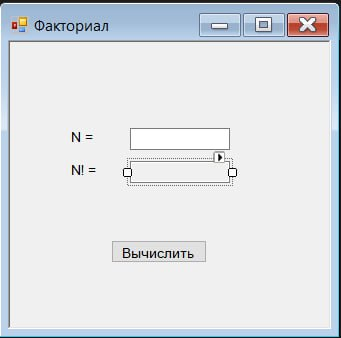
\includegraphics{../img/factorial/factorial_form.png}
    \caption{Вид формы программы вычисления факториала}
    \label{fig:factorial_form}
\end{figure}

У элементов формы изменены значения некоторых свойств \cite{microsoft_create}.
Значения измененных атрибутов представлены в таблице \ref{table:factorial_params}.

\begin{table}[H]
    \small
    \caption{Значения атрибутов элементов формы}
    \begin{tabular}{|l|l|}\hline
    Свойство & Значение\cr\hline
    \multicolumn{2}{|l|}{Форма}\cr\hline
    \verb"Text" & \verb"Факториал"\cr\hline
    \verb"FormBorderStyle" & \verb"Fixed3D"\cr\hline
    \verb"MaximizeBox" & \verb"False"\cr\hline
    \multicolumn{2}{|l|}{Первая надпись}\cr\hline
    \verb"(Name)" & \verb"label_input"\cr\hline
    \verb"Text" & \verb"N ="\cr\hline
    \multicolumn{2}{|l|}{Вторая надпись}\cr\hline
    \verb"(Name)" & \verb"label_output"\cr\hline
    \verb"Text" & \verb"N! ="\cr\hline
    \multicolumn{2}{|l|}{Первое текстовое поле}\cr\hline
    \verb"(Name)" & \verb"text_input"\cr\hline
    \multicolumn{2}{|l|}{Второе текстовое поле}\cr\hline
    \verb"(Name)" & \verb"text_output"\cr\hline
    \verb"ReadOnly" & \verb"True"\cr\hline
    \multicolumn{2}{|l|}{Кнопка}\cr\hline
    \verb"(Name)" & \verb"btn_compute"\cr\hline
    \verb"Text" & \verb"Вычислить"\cr\hline
    \multicolumn{2}{|l|}{Обработчик ошибок}\cr\hline
    \verb"(Name)" & \verb"errorProvider1"\cr\hline
    \end{tabular}
    \label{table:factorial_params}
\end{table}

Для работы программы был создан отдельный файл \verb"fact.h", содержащий   
код вычисления факториала \cite{book_excs}:
\begin{minted}[linenos, style=bw, fontsize=\small, breaklines=true]{cpp}
#pragma once
long long fact(long long n)
{
    //Если n < 0, то останавливаем с кодом -1
	if (n < 0)
		return -1;
    //Если на входе 0 или 1 - возвращаем 1
	else if (n == 0 || n == 1)
		return 1;
    //Иначе осуществляем рекурсивный вызов
	else 
		return n * fact(n - 1);
}
\end{minted}
Переменная \verb|n| "--- число, для которого вычисляется факториал.

По нажатию кнопки <<Вычислить>> происходит выполнение следующего кода:
\begin{minted}[linenos, style=bw, fontsize=\small, breaklines=true]{cpp}
private: System::Void btn_compute_Click(System::Object^ sender, System::EventArgs^ e) {
    this->text_output->Text = "";
    long long input;
    bool result = Int64::TryParse(this->text_input->Text, input);
    //Если удалось прочитать число, то вычисляем 
    //факториал.
    if (result)
    {
      long long output = fact(input);
      this->text_output->Text = System::Convert::ToString(output);
    }
    //В противном случае, с помощью ErrorProvider возвращаем ошибку.
    else
      errorProvider1->SetError(text_input, "Некорректные данные");
\end{minted}

В случае корректных входных данных, программа посчитает факториал и выведет в 
\verb|text_output| (см. рисунок \ref{fig:factorial_result}).
\begin{figure}[H]
    \centering
    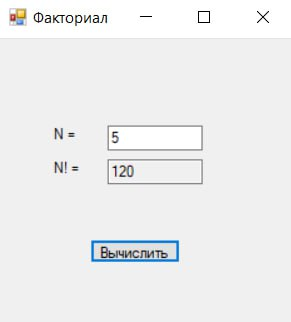
\includegraphics{../img/factorial/factoral_result.png}
    \caption{<<Факториал>>: работа программы}
    \label{fig:factorial_result}
\end{figure}

\newpage
В случае некорректных данных на входе, программа вернёт ошибку с помощью элемента 
\verb|errorProvider1| (см. рисунок \ref{fig:factorial_error}).
\begin{figure}[H]
    \centering
    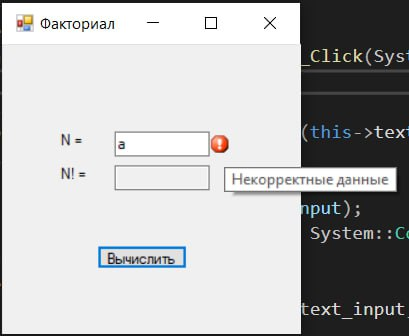
\includegraphics{../img/factorial/factorial_error.png}
    \caption{<<Факториал>>: обработка ошибок}
    \label{fig:factorial_error}
\end{figure}

С полным кодом программы можно ознакомиться в приложении \ref{app:repo}.

\section{Обработка табличных данных}
\verb|Задание.| Все столбцы, содержащие минимальный элемент, заменить столбцом X.

Создано окно приложения, содержащее три элемента \verb|DataGridView| и три элемента 
\verb|Button|. Для перехвата и обработки ошибок добавлен элемент \verb|ErrorProvider|
(см. рисунок \ref{fig:dgv_form}). 

\begin{figure}[H]
    \centering
    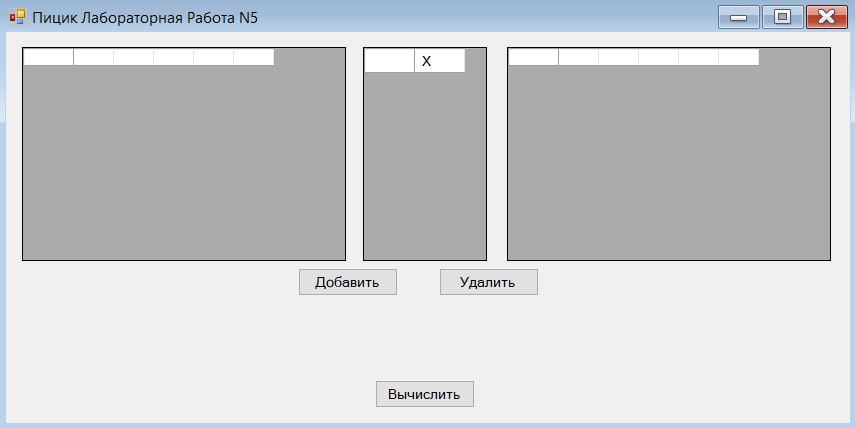
\includegraphics[scale=0.68]{../img/dgv/dgv_form.png}   
    \caption{Вид формы программы замены столбцов}
    \label{fig:dgv_form}
\end{figure}

У элементов формы изменены значения некоторых свойств, значения измененных атрибутов 
можно увидеть в таблице \ref{tab:dgv_params}.

\begin{table}[H]
    \small
    \caption{Значения атрибутов элементов формы}
    \begin{tabular}{|l|l|}\hline
    Свойство & Значение \cr\hline
    \multicolumn{2}{|l|}{Форма}\cr\hline
    \verb"Text" & Пицик Лабораторная работа N5 \cr\hline
    \multicolumn{2}{|l|}{Кнопка "Добавить"}\cr\hline
    \verb"(Name)" & btn\_add \cr\hline 
    \verb"Text" & Добавить \cr\hline 
    \multicolumn{2}{|l|}{Кнопка "Удалить"}\cr\hline
    \verb"(Name)" & btn\_rm\cr\hline
    \verb"Text" & Удалить \cr\hline
    \multicolumn{2}{|l|}{Кнопка "Вычислить"}\cr\hline
    \verb"(Name)" & btn\_calc \cr\hline 
    \verb"Text" & Вычислить \cr\hline
    \multicolumn{2}{|l|}{DataGridView для ввода}\cr\hline
    \verb"(Name)" & data\_first\cr\hline
    \verb"AllowUserToAddRows" & False\cr\hline
    \verb"AllowUserToDeleteRows" & False\cr\hline
    \multicolumn{2}{|l|}{DataGridView для столбца X}\cr\hline
    \verb"(Name)" & data\_x \cr\hline
    \verb"AllowUserToAddRows" & False\cr\hline
    \verb"AllowUserToDeleteRows" & False\cr\hline
    \multicolumn{2}{|l|}{DataGridView для вывода}\cr\hline
    \verb"(Name)" & data\_result \cr\hline
    \verb"AllowUserToAddRows" & False\cr\hline
    \verb"AllowUserToDeleteRows" & False\cr\hline
    \verb"ColumnHeadersHeightSizeMode" & AutoSize \cr\hline
    \verb"ReadOnly" & True \cr\hline
    \multicolumn{2}{|l|}{Обработчик ошибок}\cr\hline
    \verb"(Name)" & error\_prov \cr\hline
    \end{tabular}
    \label{tab:dgv_params}
\end{table}

С помощью параметров столбцов элемента \verb|DataGridView|, контекстное меню которых можно 
вызвать, нажав на стрелочку около элемента и на свойство <<Правка столбцов>>, у элемента 
\verb|data_x| было добавлено название столбца <<X>> \cite{book_msvisual}.

Для добавления столбцов, в кнопке <<Добавить>> был разработан следующий код \cite{book_tmp}:
\begin{minted}[linenos, style=bw, fontsize=\small, breaklines=true]{cpp}
private: System::Void btn_add_Click(System::Object^ sender, System::EventArgs^ e) 
  {
    data_first->Rows->Add();
    data_x->Rows->Add();
    data_result->Rows->Add();
  }
\end{minted}

Для удаления столбцов, в кнопке <<Удалить>> был разработан следующий код:
\begin{minted}[linenos, style=bw, fontsize=\small, breaklines=true]{cpp}
private: System::Void btn_rm_Click(System::Object^ sender, System::EventArgs^ e) {
  if (data_first->CurrentRow != nullptr && !data_first->CurrentRow->IsNewRow)
  {
    int rowIndex = data_first->CurrentRow->Index;

    if (rowIndex < data_first->Rows->Count)
    // удаляем строку из data_first
    data_first->Rows->RemoveAt(rowIndex);

    // проверяем есть ли rowIndex в data_x
    if (rowIndex < data_x->Rows->Count)
      // удаляем строку из data_x по тому же индексу
      data_x->Rows->RemoveAt(rowIndex);

    // проверяем есть ли rowIndex в data_result
    if (rowIndex < data_result->Rows->Count)
      // удаляем строку из data_result по тому же индексу
      data_result->Rows->RemoveAt(rowIndex);
  }
}
\end{minted}
В переменную \verb|rowIndex| записывается индекс выбранной строки \verb|DataGridView|.
Затем, для предотвращения ошибок, перед удалением строки из каждого элемента \verb|DataGridView|,
производится проверка, что индекс выбранной строки не превышает общее количество строк каждого элемента.
Затем, если условие соблюдается, осуществляется удаление строк.

Для корректного отображения ошибок, была реализована вспомогательная функция \verb|ClearAll()|:
\begin{minted}[linenos, style=bw, fontsize=\small, breaklines=true]{cpp}
void ClearAll()
{
    error_prov->SetError(btn_calc, "");
}
\end{minted}

С остальными кодами можно ознакомиться в приложении \ref{app:codes}.

При запуске приложения открывается окно(см. рисунок \ref{fig:dgv_onlaunch}).

\begin{figure}[H]
\centering
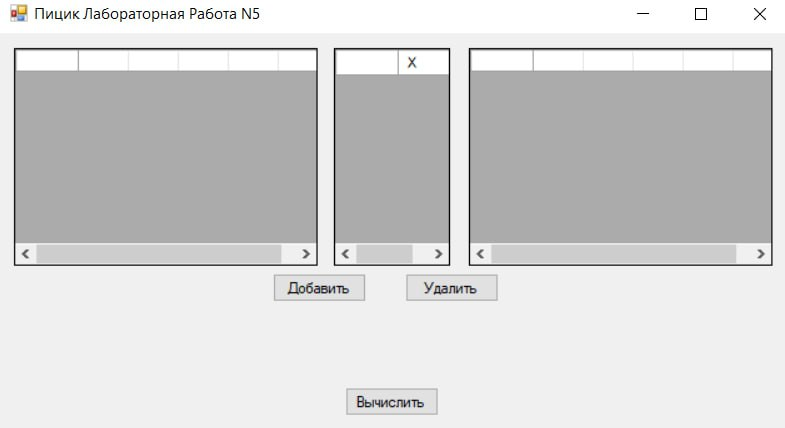
\includegraphics[scale=.65]{../img/dgv/dgv_on_launch.jpg}
\caption{<<Табличные данные>>: звпуск программы}
\label{fig:dgv_onlaunch}
\end{figure}

Ввод некорректных данных обрабатывается с помощью \verb|ErrorProvider| и сопровождается 
выводом сообщения об ошибке (см. рисунок \ref{fig:dgv_error}). 
\begin{figure}[H]
    \centering
    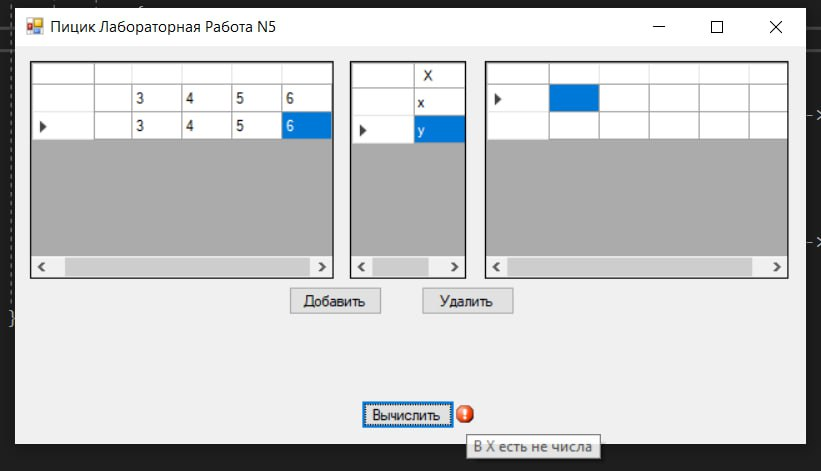
\includegraphics[scale=0.68]{../img/dgv/dgv_error.png}
    \caption{<<Табличные данные>>: сообщение об ошибке}
    \label{fig:dgv_error}
\end{figure}

Пример корректной работы программы изображен на рисунке \ref{fig:dgv_result}. 
\begin{figure}[H]
    \centering
    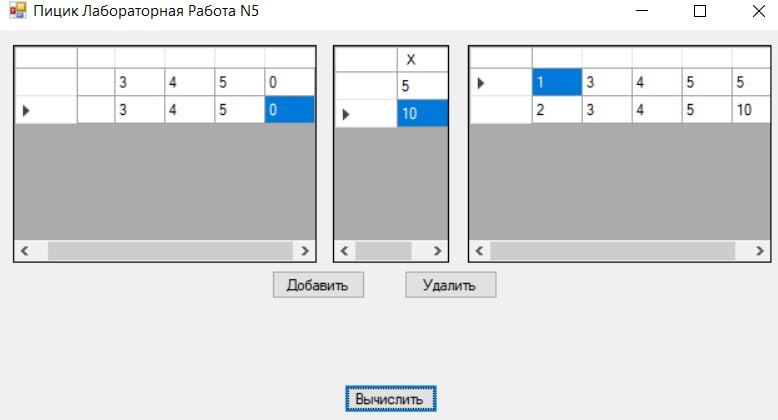
\includegraphics[scale=0.68]{../img/dgv/dgv_result.png}
    \caption{<<Табличные данные>>: работа программы}
    \label{fig:dgv_result}
\end{figure}

Полный код программы приведён в приложении \ref{app:repo}. 
\section{Использование коллекций в Windows Forms}
\verb|Задание.| Создать словарь, состоящий из строк. В качестве ключа выступает фамилия, 
в качестве значения — должность. Вывести на экран фамилии людей, занимающих данную должность. 
Вывести должность, занимаемую данным \newline человеком.

Для выполнения данного задания была создана форма, содержащая один элемент \verb|DataGridView|, 
три элемента \verb|Label|, четыре элемента \verb|TextBox| и три элемента \verb|Button| (см. рисунок 
\ref{fig:col_form}). 
\begin{figure}[H]
    \centering
    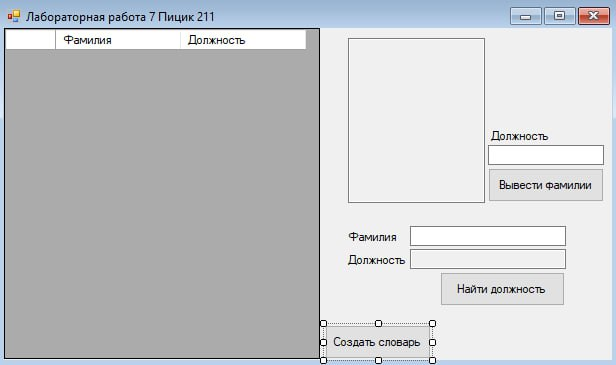
\includegraphics[scale=0.68]{../img/collections/collections_form.png}
    \caption{Вид формы программы обработки отсортированного словаря}
    \label{fig:col_form}
\end{figure}

У элементов формы изменены значения некоторых свойств. С полным списком измененных свойств 
можно ознакомиться в таблице \ref{tab:col_params}.

\begin{table}[H]
    \small
    \caption{Значения атрибутов элементов формы}
    \begin{tabular}{|l|l|}\hline
    Свойство & Значение \cr\hline
    \multicolumn{2}{|l|}{Форма}\cr\hline
    \verb"Text" & Лабораторная Работа 7 Пицик 211 \cr\hline
    \multicolumn{2}{|l|}{Верхняя надпись <<Должность>>}\cr\hline
    \verb"(Name)" & label\_work1 \cr\hline
    \verb"Text" & Должность \cr\hline
    \multicolumn{2}{|l|}{Надпись <<Фамилия>>}\cr\hline
    \verb"(Name)" & label\_surname \cr\hline
    \verb"Text" & Фамилия \cr\hline
    \multicolumn{2}{|l|}{Нижняя надпись <<Должность>>}\cr\hline
    \verb"(Name)" & label\_work \cr\hline
    \verb"Text" & Должность \cr\hline
    \multicolumn{2}{|l|}{Текстовое поле для ввода должности} \cr\hline
    \verb"(Name)" & text\_work1 \cr\hline
    \multicolumn{2}{|l|}{Текстовое поле для вывода фамилий} \cr\hline
    \verb"(Name)" & text\_list \cr\hline
    \verb"ReadOnly" & True \cr\hline
    \verb"Multiline" & True \cr\hline
    \multicolumn{2}{|l|}{Текстовое поле для ввода фамилии} \cr\hline
    \verb"(Name)" & text\_surname \cr\hline
    \multicolumn{2}{|l|}{Текстовое поле для вывода должности} \cr\hline
    \verb"(Name)" & text\_work \cr\hline
    \verb"ReadOnly" & True \cr\hline
    \multicolumn{2}{|l|}{Кнопка <<Создать словарь>>}\cr\hline
    \verb"(Name)" & btn\_dict \cr\hline 
    \verb"Text" & Создать словарь \cr\hline 
    \multicolumn{2}{|l|}{Кнопка <<Вывести фамилии>>}\cr\hline
    \verb"(Name)" & btn\_list\cr\hline
    \verb"Text" & Вывести фамилии \cr\hline
    \multicolumn{2}{|l|}{Кнопка <<Найти должность>>}\cr\hline
    \verb"(Name)" & btn\_find \cr\hline 
    \verb"Text" & Найти должность \cr\hline
    \multicolumn{2}{|l|}{DataGridView для колллекции}\cr\hline
    \verb"(Name)" & dgv\_table\cr\hline
    \verb"AllowUserToAddRows" & False\cr\hline
    \verb"AllowUserToDeleteRows" & False\cr\hline
    \verb"ReadOnly" & True\cr\hline
    \end{tabular}
    \label{tab:col_params}
\end{table}

С помощью свойства \verb|Enabled| элемента \verb|button_dict| осуществляется запрет 
на повторное нажание кнопки \cite{microsoft_enabled}. Создание словаря осуществляется с помощью следующего кода:
\begin{minted}[linenos, breaklines=true, fontsize=\small, style=bw]{cpp}
System::Collections::Generic::SortedDictionary <String^, String^> dict;
\end{minted}
Здесь \verb|dict| "--- название переменной, которое будет иметь отсортированный словарь.
Основные свойства и методы словаря описаны в таблице \ref{tab:col_methods} \cite{microsoft_dict}.

\begin{table}[H]
    \small
    \caption{Свойства и методы словаря}
    \begin{tabular}{|l|l|}\hline
    \multicolumn{2}{|l|}{Свойства}\cr\hline
    \verb"dict.Count()" & возвращает количество элементов словаря \cr\hline
    \verb"dict.Keys()" & возвращает коллекцию, содержащую ключи словаря \cr\hline
    \verb"dict.Values()" & возвращает коллекцию, содержащую значения словаря \cr\hline
    \multicolumn{2}{|l|}{Методы}\cr\hline
    \verb"dict.Clear()" & очистка словаря \cr\hline
    \verb"dict.Add(X)" & добавление нового элемента в словарь \cr\hline
    \verb"dict.ContainsKey(X)" & возвращает \verb|true|, если ключ X есть в словаре \cr\hline
    \verb"dict.ContainsValue(X)" & возвращает \verb|true|, если значение X есть в словаре \cr\hline
    \verb"dict.Remove(X)" & удаляет элемент X \cr\hline
    \verb"dict.TryGetValue(X)" & возвращает \verb|true|, если ключ X есть в словаре и возвращает значение\cr\hline
    \end{tabular}
    \label{tab:col_methods}
\end{table}

Код кнопки <<Создать словарь>> выглядит следующим образом:
\begin{minted}[linenos, breaklines=true, style=bw, fontsize=\small]{cpp}
private: System::Void btn_dict_Click(System::Object^ sender, System::EventArgs^ e) {
    this->btn_dict->Enabled = false;
    System::Collections::Generic::SortedDictionary <String^, String^> dict;
    
    //Элементы словаря
    dict.Add("Пицик", "Старший разработчик");
    dict.Add("Коновалов", "DevOps инженер");
    dict.Add("Дрождев", "Разработчик");
    dict.Add("Цой", "ML-инженер");
    dict.Add("Артамонова", "Средний разработчик");
    dict.Add("Карасёв", "DevOps инженер");
    dict.Add("Воронцов", "Prompt инженер");
    dict.Add("Гришин", "Full-stack разработчик");
    dict.Add("Николаев", "GameDev разработчик");
    dict.Add("Иванов", "Младший разработчик");

    for each (KeyValuePair<String^, String^> item in dict)
    {
      int row = dgv_table->Rows->Add();
      dgv_table->Rows[row]->Cells[0]->Value = item.Key;
      dgv_table->Rows[row]->Cells[1]->Value = item.Value;
    }
  }
\end{minted}
Создаётся словарь \verb|dict|, заполняется с помощью метода \verb|dict.Add()|, а затем 
элементы словаря переносятся в окно элемента \verb|dgv_table| \cite{microsoft_dgv}.
Для корректной работы \verb|KeyValuePair| необходимо разрешить пространство имён \verb|Generic|:
\begin{minted}[linenos, breaklines=true, fontsize=\small, style=bw]{cpp}
using namespace System::Collections::Generic;
\end{minted}

С остальными кодами можно ознакомиться в приложении \ref{app:codes}.

При открытии приложения появляется окно (см. рисунок \ref{fig:cols_res}).
\begin{figure}[H]
  \centering
  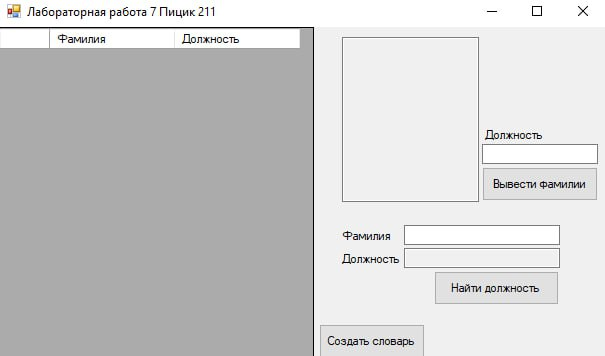
\includegraphics[scale=.85]{../img/collections/collections_res.jpg}
  \caption{Окно приложения <<Коллекции>>: начальный запуск}
  \label{fig:cols_res}
\end{figure}

При нажатии кнопки <<Создать словарь>> обновляется содержимое \newline \verb|DataGidView|
(см. рисунок \ref{fig:cols_create}).
\begin{figure}[H]
  \centering
  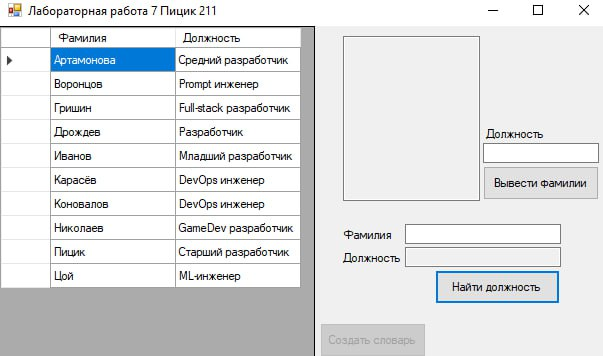
\includegraphics[scale=.85]{../img/collections/collections_create.jpg}
  \caption{<<Коллекции>>: создание словаря}
  \label{fig:cols_create}
\end{figure}

При поиске фамилий по должности или должности по фамилии и корректном вводе данных, 
выводится соответствующий результат как показано на рисунке \ref{fig:cols_find}.
\begin{figure}[H]
  \centering
  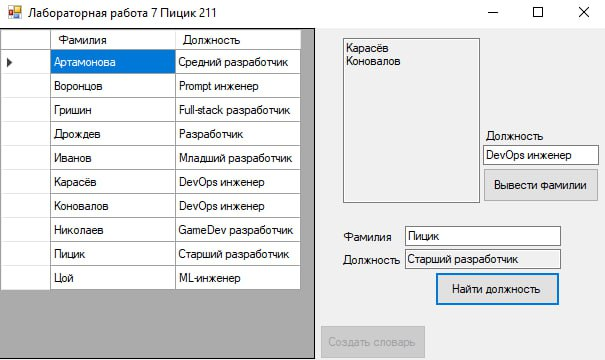
\includegraphics[scale=.85]{../img/collections/collections_find.jpg}
  \caption{<<Коллекции>>: поиск при корректных данных}
  \label{fig:cols_find}
\end{figure}

При поиске с некорректными данными, выводятся соответствующие ошибки 
(см. рисунок \ref{fig:cols_error}).
\begin{figure}[H]
  \centering
  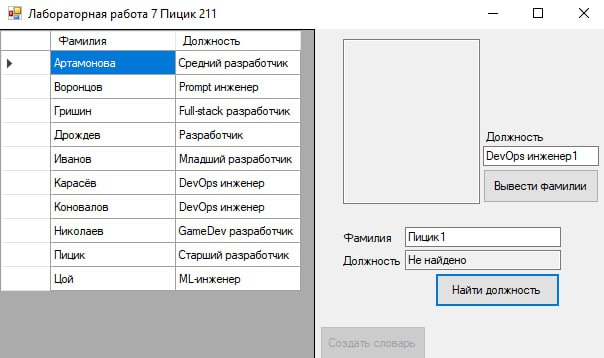
\includegraphics[scale=.85]{../img/collections/collections_error.jpg}
  \caption{<<Коллекции>>: вывод ошибок}
  \label{fig:cols_error}
\end{figure}

Полный код программы доступен в приложении \ref{app:repo}.
\section{Файловые диалоги и работа с файлами}
\verb|Задание.| Создать таблицу Student. В другой файл вывести студентов, у которых сдана сессия. (Вариант 1)

Для выполнения данного задания была разработна форма, содержащая два элемента 
\verb|DataGridView|, шесть элементов \verb|Button|, элементы \verb|OpenFileDialog| и \verb|SaveFileDialog| для 
работы с файлами, и элемент \verb|ErrorProvider| (см. рисунок \ref{fig:files_const}).

\begin{figure}[H]
\centering
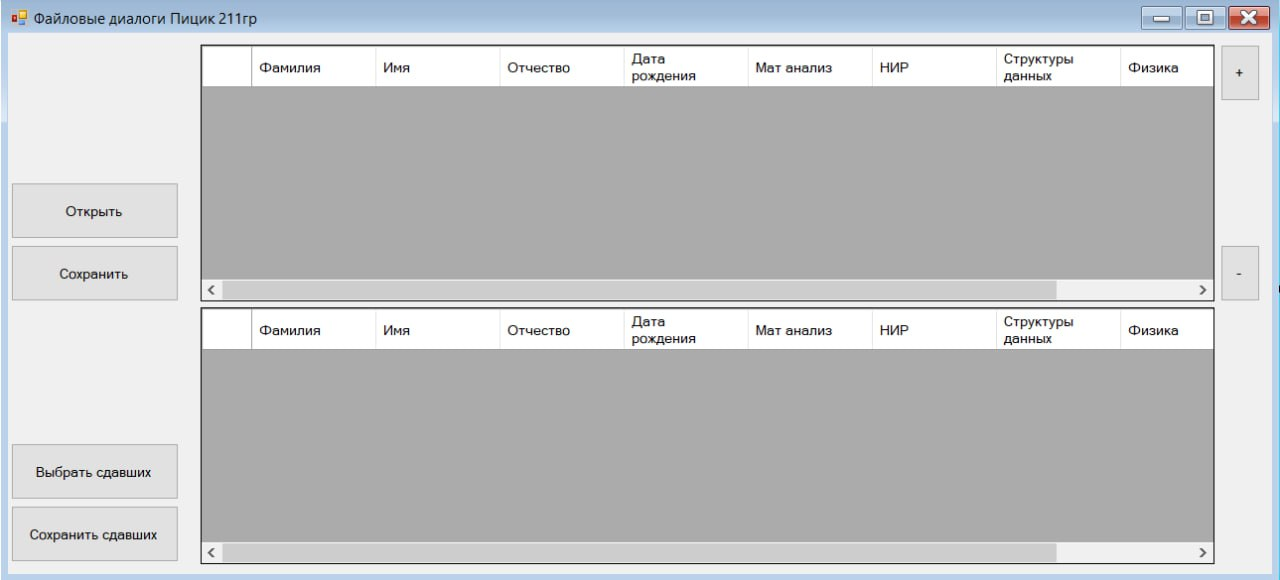
\includegraphics[scale=.45]{../img/files/files_konstructor.jpg}
\caption{Итоговый вид окна}
\label{fig:files_const}
\end{figure}

У элементов формы изменены значения некоторых свойств. С полным списком 
измененных свойств можно ознакомиться в таблице \ref{tab:files}.

\begin{table}[H]
    \small
    \caption{Значение атрибутов элементов формы}
    \begin{tabular}{|l|l|}\hline
        \multicolumn{2}{|l|}{Форма}\cr\hline
        \verb"Text" & Файловые диалоги Пицик 211гр.\cr\hline
        \multicolumn{2}{|l|}{DataGridView для ввода}\cr\hline
        \verb"(Name)" & data\_inuput\cr\hline
        \verb"AllowUserToAddRows" & False\cr\hline
        \verb"AllowUserToDeleteRows" & False\cr\hline
        \multicolumn{2}{|l|}{DataGridView для вывода}\cr\hline
        \verb"(Name)" & data\_output \cr\hline
        \verb"AllowUserToAddRows" & False\cr\hline
        \verb"AllowUserToDeleteRows" & False\cr\hline
        \multicolumn{2}{|l|}{Кнопка <<Открыть>>}\cr\hline
        \verb"(Name)" & btn\_open \cr\hline
        \verb"Text" & Открыть \cr\hline
        \multicolumn{2}{|l|}{Кнопка <<Сохранить>>}\cr\hline
        \verb"(Name)" & btn\_save \cr\hline
        \verb"Text" & Сохранить \cr\hline
        \multicolumn{2}{|l|}{Кнопка <<Выбрать сдавших>>}\cr\hline
        \verb"(Name)" & btn\_choose \cr\hline
        \verb"Text" & Выбрать сдавших \cr\hline
        \multicolumn{2}{|l|}{Кнопка <<Сохранить сдавших>>}\cr\hline
        \verb"(Name)" & btn\_savechoose \cr\hline
        \verb"Text" & Сохранить сдавших\cr\hline
        \multicolumn{2}{|l|}{Кнопка <<+>>}\cr\hline
        \verb"(Name)" & btn\_add \cr\hline
        \verb"Text" & + \cr\hline
        \multicolumn{2}{|l|}{Кнопка << - >>}\cr\hline
        \verb"(Name)" & btn\_remove \cr\hline
        \verb"Text" & - \cr\hline
        \multicolumn{2}{|l|}{Файловые диалог <<Открыть>>}\cr\hline
        \verb"(Name)" & open\_fd \cr\hline
        \verb"Title" & Открыть файл \cr\hline
        \verb"Filter" & Текстовые файлы (*.txt) | *.txt | Все файлы (*.*) | *.*\cr\hline
        \multicolumn{2}{|l|}{Файловые диалог <<Сохранить>>}\cr\hline
        \verb"(Name)" & save\_fd \cr\hline
        \verb"Title" & Сохранить файл \cr\hline
        \verb"Filter" & Текстовые файлы (*.txt) | *.txt | Все файлы (*.*) | *.*\cr\hline
    \end{tabular}
    \label{tab:files}
\end{table}

При нажатии кнопки <<Открыть>> открывается окно, позволяющее выбрать файлы форматов, заданных 
в свойстве \verb|Filter| для элемента \verb|OpenFileDialog| (см. рисунок \ref{fig:files_open}) \cite{book_beginners}.

\begin{figure}[H]
\centering
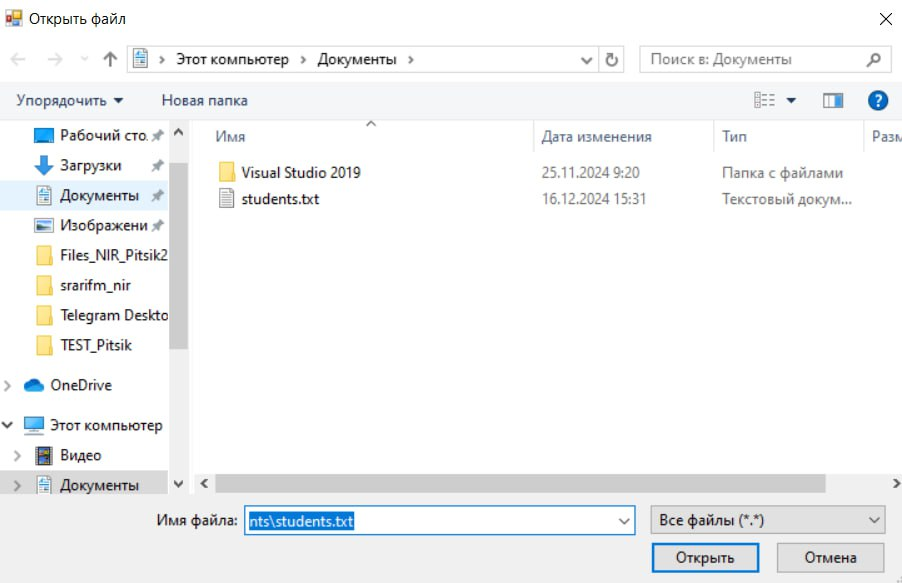
\includegraphics[scale=.65]{../img/files/files_open.jpg}
\caption{Открытие файла}
\label{fig:files_open}
\end{figure}

Для кнопнки <<Открыть>> был разработан следующий код:
\begin{minted}[linenos, breaklines=true, style=bw, fontsize=\small]{cpp}
private: System::Void btn_open_Click(System::Object^ sender, System::EventArgs^ e) {
    error_prov->Clear();

//открываем поток 
    System::IO::Stream^ myStream;
    if (this->openFileDialog->ShowDialog() == System::Windows::Forms::DialogResult::OK)
  //если успешно найден файл
      if ((myStream = openFileDialog->OpenFile()) != nullptr)
      {
//задаем кодировку чтения
        System::IO::StreamReader^ sr = gcnew System::IO::StreamReader(
          myStream, System::Text::Encoding::GetEncoding(1251)
        );
//заполняем dgv
        int row = 0;
        System::String^ str1 = "";
        while (sr->Peek() > -1)
        {
          str1 = sr->ReadLine();
          array<String^>^ words = str1->Split(' ');
          dgv_input->Rows->Add(words);
        }
//закрываем поток
        sr->Close();
      }
  }
\end{minted}

В случае сохранения файла, необходимо нажать кнопку <<Сохранить>>, фрагмент кода которой представлен ниже \cite{book_gui}.
\begin{minted}[linenos, breaklines=true, fontsize=\small, style=bw]{cpp}
System::IO::Stream^ myStream;
//открываем окно сохранения файла
      if (this->saveFileDialog->ShowDialog() == System::Windows::Forms::DialogResult::OK)
      {
        if ((myStream = saveFileDialog->OpenFile()) != nullptr)
        {
//запись файла
          System::IO::StreamWriter^ sw = gcnew System::IO::StreamWriter(myStream, System::Text::Encoding::GetEncoding(1251));
//считываем с итоговой таблицы
          for (int i = 0; i < dgv_output->RowCount; ++i)
          {
            String^ s;
            for (int j = 0; j < dgv_output->ColumnCount; ++j)
              s += System::Convert::ToString(dgv_output->Rows[i]->Cells[j]->Value) + " ";
//записываем строку
            sw->WriteLine(s);
          }
//закрываем поток
          sw->Close();
        }
      }
\end{minted}

С остальными кодами можно ознакомиться в приложении \ref{app:codes}.

При запуске программы открывается окно (см. рисунок \ref{fig:files_res}).
\begin{figure}[H]
\centering
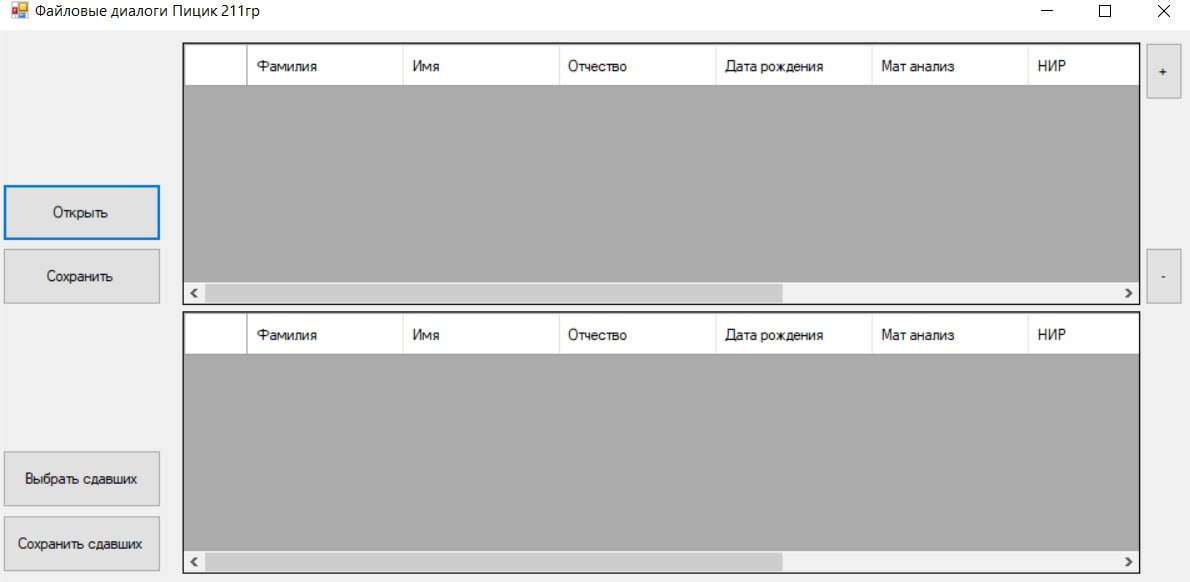
\includegraphics[scale=.45]{../img/files/files_res.jpg}
\caption{Окно приложения <<Файловые диалоги>>: запуск программы}
\label{fig:files_res}
\end{figure}

При нажатии на кнопку <<Выбрать сдавших>> в нижний элемент \verb|DataGridView| выводится список 
сдавших студентов (см. рисунок \ref{fig:files_choose}).
\begin{figure}[H]
\centering
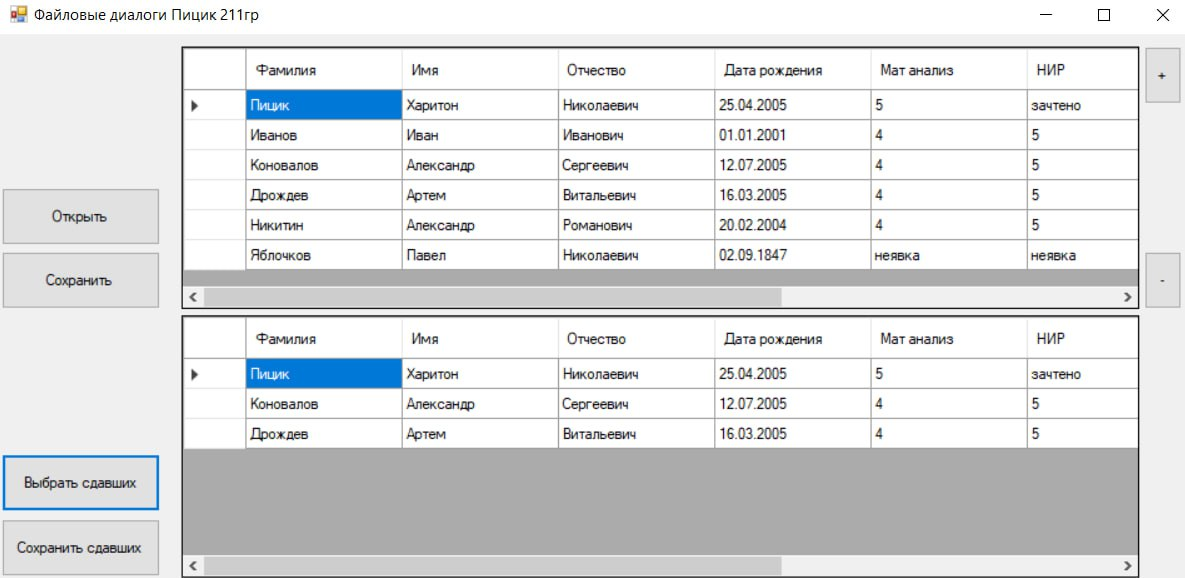
\includegraphics[scale=.45]{../img/files/files_choose.jpg}
\caption{<<Файловые диалоги>>: вид окна после выбора сдавших}
\label{fig:files_choose}
\end{figure}

При попытке добавить в исходную таблицу строку, содержащую некорректное значение даты или оценки, выводится ошибка 
(см. рисунок \ref{fig:files_error}).
\begin{figure}[H]
\centering
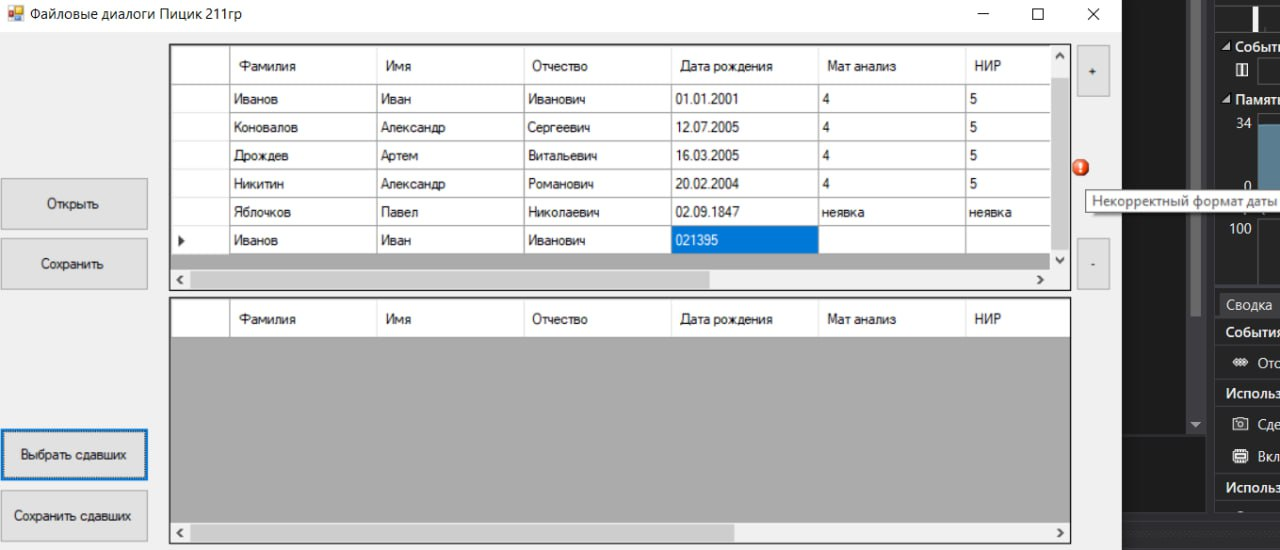
\includegraphics[scale=.45]{../img/files/files_error.jpg}
\caption{<<Файловые диалоги>>: вывод ошибки в окне программы}
\label{fig:files_error}
\end{figure}

Полный код программы приведён в приложении \ref{app:repo}.
\section{Приложение ТЕСТ}
\verb|Задание.| Создать приложение для проведения тестирования. \newline Должно содержать:
\begin{enumerate}
    \item Набор вопросов по какой-то теме (и вопросы и ответы должны быть реальные) "--- не менее 10
    \item Вопросы должны выбираться случайным образом.
    \item Вопросы должны быть нескольких типов "--- "Да/нет", Выбор одного ответа, Выбор нескольких ответов, Короткий ответ.
    \item Необходимо создать сообщения для правильного и неправильного ответа (Молодец, Не правильно и т.д.)
    \item Необходимо подсчитать количество правильных ответов и вывести результат.
\end{enumerate}

Для выполнения данного задания была разработана форма, содержащая два элемента 
\verb|TextBox|, четыре элемента \verb|GroupBox|, шесть элементов \verb|RadioButton|, 
четыре элемента \verb|CheckBox| и один элемент \verb|Button| (см. рисунок \ref{fig:test_const}).
\begin{figure}[H]
\centering
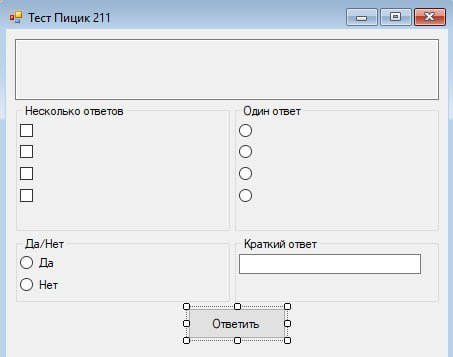
\includegraphics[scale=.85]{../img/test/test_const.jpg}
\caption{Окно приложения <<Тест>> открытое в конструкторе}
\label{fig:test_const}
\end{figure}

У элементов формы изменены значения некоторых свойств. Значения изменённых атрибутов 
представлены в таблицах \ref{tab:test} и \ref{tab:test_1}.
\begin{table}[H]
    \small
    \caption{Значение артибутов элементов формы, часть 1}
    \begin{tabular}{|l|l|}\hline
        \multicolumn{2}{|l|}{Форма}\cr\hline
        \verb"Text" & Тест Пицик 211 \cr\hline
        \multicolumn{2}{|l|}{Окно вывода вопросов}\cr\hline
        \verb"(Name)" & text\_questions \cr\hline
        \verb"ReadOnly" & True \cr\hline
        \multicolumn{2}{|l|}{Группа для нескольких ответов}\cr\hline
        \verb"(Name)" & group\_multiple \cr\hline
        \verb"Text" & Несколько ответов \cr\hline
        \multicolumn{2}{|l|}{Несколько ответов: 1"=й вариант}\cr\hline
        \verb"(Name)" & check\_1 \cr\hline
        \verb"Text" & \cr\hline
        \multicolumn{2}{|l|}{Несколько ответов: 2"=й вариант}\cr\hline
        \verb"(Name)" & check\_2 \cr\hline
        \verb"Text" & \cr\hline
        \multicolumn{2}{|l|}{Несколько ответов: 3"=й вариант}\cr\hline
        \verb"(Name)" & check\_3 \cr\hline
        \verb"Text" & \cr\hline
        \multicolumn{2}{|l|}{Несколько ответов: 4"=й вариант}\cr\hline
        \verb"(Name)" & check\_4 \cr\hline
        \verb"Text" & \cr\hline
        \multicolumn{2}{|l|}{Группа для одного ответа}\cr\hline
        \verb"(Name)" & group\_single \cr\hline
        \verb"Text" & Один ответ \cr\hline
        \multicolumn{2}{|l|}{Один ответ: 1"=й вариант}\cr\hline
        \verb"(Name)" & radio\_single1 \cr\hline
        \verb"Text" & \cr\hline
        \multicolumn{2}{|l|}{Один ответ: 2"=й вариант}\cr\hline
        \verb"(Name)" & radio\_single2 \cr\hline
        \verb"Text" & \cr\hline
        \multicolumn{2}{|l|}{Один ответ: 3"=й вариант}\cr\hline
        \verb"(Name)" & radio\_single3 \cr\hline
        \verb"Text" & \cr\hline
        \multicolumn{2}{|l|}{Один ответ: 4"=й вариант}\cr\hline
        \verb"(Name)" & radio\_single4 \cr\hline
        \verb"Text" & \cr\hline
    \end{tabular}
    \label{tab:test}
\end{table}

\begin{table}[H]
\small
\caption{Значение артибутов элементов формы, часть 2}
\begin{tabular}{|l|l|}\hline
    \multicolumn{2}{|l|}{Группа для Да/Нет}\cr\hline
    \verb"(Name)" & group\_yesno \cr\hline
    \verb"Text" & Да/нет \cr\hline
    \multicolumn{2}{|l|}{Да/нет: да}\cr\hline
    \verb"(Name)" & radio\_yes \cr\hline
    \verb"Text" & Да \cr\hline
    \multicolumn{2}{|l|}{Да/нет: нет}\cr\hline
    \verb"(Name)" & radio\_no \cr\hline
    \verb"Text" & Нет \cr\hline
    \multicolumn{2}{|l|}{Группа для краткого ответа}\cr\hline
    \verb"(Name)" & group\_txt \cr\hline
    \verb"Text" & Краткий ответ \cr\hline
    \multicolumn{2}{|l|}{Краткий ответ: текст}\cr\hline
    \verb"(Name)" & text\_answer \cr\hline
    \multicolumn{2}{|l|}{Кнопка для ответа}\cr\hline
    \verb"(Name)" & btn\_answer \cr\hline
    \verb"Text" & Ответить \cr\hline
\end{tabular}
\label{tab:test_1}
\end{table}

Были созданы отдельные структуры для отслеживания типа вопроса, \newline вариантов ответа и правильного ответа:
\begin{minted}[linenos, breaklines=true, style=bw, fontsize=\small]{cpp}
// структура для Теста
public enum struct Test
    {
        yes_no,
        single,
        multiple,
        txt_answer
    };

    //структура вопросов
    public ref struct Questions
    {
        System::String^ text; //формулировка вопроса
        array<System::String^>^ answers; //варианты ответа
        Test type; //тип ответа
        System::Object^ answer; //ответ 
    };
\end{minted}

Была создана отдельная функция для перемешивания всех вопросов:
\begin{minted}[linenos, breaklines=true, fontsize=\small, style=bw]{cpp}
// функция для перемешивания вопросов
void randomize_questions(array<Questions^>^ arr) {
        Random^ rand = gcnew Random();
        for (int i = arr->Length - 1; i > 0; --i)
        {
            int j = rand->Next(0, i + 1);

            Questions^ temp = arr[i];
            arr[i] = arr[j];
            arr[j] = temp;
        }
    }
\end{minted}

Фрагмент массива, содержащего все вопросы для теста:
\begin{minted}[linenos, style=bw, fontsize=\small, breaklines=true]{cpp}
//массив всех вопросов 
array<Questions^>^ test_dataset() {
    array<Questions^>^ q = gcnew array<Questions^>(12);

    q[0] = gcnew Questions();
    q[0]->text = "C++, Python, C - это всё ______ (полное словосочетание)";
    q[0]->type = Test::txt_answer;
    q[0]->answer = "языки программирования";

    q[1] = gcnew Questions();
    q[1]->text = "Какой тип данных описывает целочисленный тип?";
    q[1]->type = Test::single;
    q[1]->answers = gcnew array<String^>{ "integer", "float", "boolean", "string" };
    q[1]->answer = 0;
\end{minted}

С остальными кодами можно ознакомиться в приложении \ref{app:codes}.

После запуска приложения появляется окно (см. рисунок \ref{fig:test_res}).
\begin{figure}[H]
    \centering
    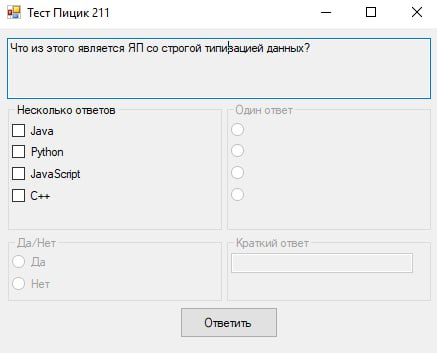
\includegraphics[scale=.85]{../img/test/test_res.jpg}
    \caption{Окно приложения <<Тест>>: начальный запуск}
    \label{fig:test_res}
\end{figure}

При выборе правильного варианта ответа появляется \verb|MessageBox| с надписью
(см. рисунок \ref{fig:test_correct}).
\begin{figure}[H]
\centering
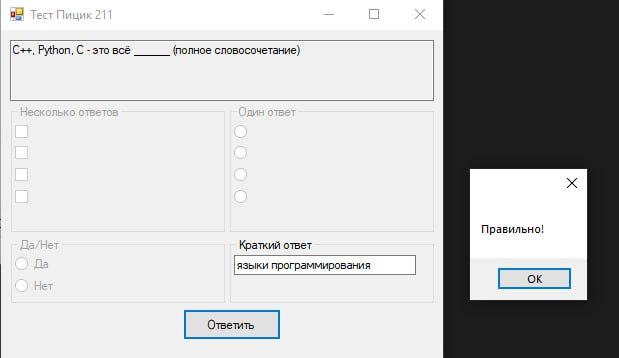
\includegraphics[scale=.85]{../img/test/test_correct.jpg}
\caption{<<Тест>>: выбор правильного ответа}
\label{fig:test_correct}
\end{figure}

При выборе неправильного варианта, выводится другое сообщение (см. рисунок \ref{fig:test_incorrect}).
\begin{figure}[H]
    \centering
    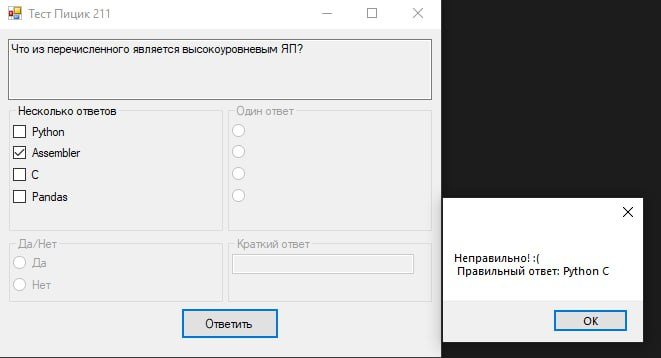
\includegraphics[scale=.85]{../img/test/test_incorrect.jpg}
    \caption{<<Тест>>: выбор неправильного ответа}
    \label{fig:test_incorrect}
\end{figure}

По прохождению теста выводится сообщение о завершении теста, а также счёт пользователя (см. рисунок \ref{fig:test_finish}).
\begin{figure}[H]
    \centering
    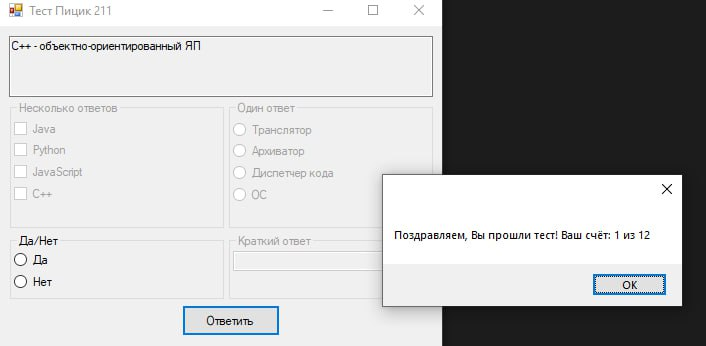
\includegraphics[scale=.85]{../img/test/test_finish.jpg}
    \caption{<<Тест>>: завершение теста}
    \label{fig:test_finish}
\end{figure}

С полным кодом программы можно ознакомиться в приложении \ref{app:repo}.

\conclusion
В ходе практики было реализовано несколько приложений на языке \verb|C++|
в среде \verb|Microsoft Visual Studio| с целью закрепления навыков построения оконного интерфейса. 
На практике разработаны приложения, содержащие такие
элементы интерфейса как \verb|TextBox|, \verb|Label|, \verb|Button|, 
\verb|DataGridView|,
\verb|OpenFileDialog|, \verb|SaveFileDialog|, \verb|ErrorProvider|.
\newpage
\bibliographystyle{gost780uv}
\bibliography{thesis}


\appendix
\section{Примеры кода} \label{app:codes}
\subsection*{Обработка табличных данных}
Код кнопки <<Вычислить>>:
\begin{minted}[linenos, breaklines=true, style=bw, fontsize=\small]{cpp}
private: System::Void btn_calc_Click(System::Object^ sender, System::EventArgs^ e) {
  ClearAll();
  if (data_x->Rows->Count != data_first->Rows->Count)
    error_prov->SetError(btn_calc, "Размерности исходной матрицы и X не совпадают!");
  else
  {
    int min_el = 1000000; //условное значение для поиска минимума
    //первый цикл - ищем минимальный элемент в принципе

    bool flag_for_data = true;
    for (int i = 0; i < data_first->Columns->Count; i++)
      for (int j = 0; j < data_first->Rows->Count; j++)
      {
        int data_el;
        bool data_fl = Int32::TryParse(System::Convert::ToString(data_first->Rows[j]->Cells[i]->Value), data_el);
        if (!data_fl)
        {
          error_prov->SetError(btn_calc, "В матрице есть не числа");
          flag_for_data = false; //исходная таблица не прошла проверку
        }
        if (data_el < min_el)
          min_el = data_el;
      }
    bool flag_for_x = true;

    //проверяем корректность данных в X
    for (int k = 0; k < data_x->Rows->Count; k++)
    {
      int x_el;
      bool x_fl = Int32::TryParse(System::Convert::ToString(data_x->Rows[k]->Cells[0]->Value), x_el);
      if (!x_fl)
      {
        //выводим ошибку
        error_prov->SetError(btn_calc, "В X есть не числа");
        flag_for_x = false;//x не прошел проверку
      }
    }
    //если все данные прошли проверку
    if (flag_for_x && flag_for_data)
    {
      bool is_swapped; //если столбец уже нужно поменять на Х
      for (int i = 0; i < data_first->Columns->Count; i++)
      {
        is_swapped = false;
        for (int j = 0; j < data_first->Rows->Count; j++)
        {
          int data_el = Int32::Parse(System::Convert::ToString(data_first->Rows[j]->Cells[i]->Value));
          if (data_el == min_el) //если в столбце найден мин. элемент
          {
            is_swapped = true; //говорим, что столбец нужно менять
            for (int k = 0; k < data_x->Rows->Count; k++)
            {
              //в результирующую таблицу вносим столбец Х
              data_result->Rows[k]->Cells[i]->Value = data_x->Rows[k]->Cells[0]->Value;
            }
            break;
          }
          //иначе вносим исходную
          if (!is_swapped) //иначе
            data_result->Rows[j]->Cells[i]->Value = data_first->Rows[j]->Cells[i]->Value;
        }
      }
    }
  }
}
\end{minted}
\subsection*{Использование коллекций в Windows Forms}
Для кнопки <<Найти должность>> разработан следующий код:
\begin{minted}[linenos, breaklines=true, style=bw, fontsize=\small]{cpp}
private: System::Void btn_find_Click(System::Object^ sender, System::EventArgs^ e) {
  String^ surname = this->text_surname->Text; //считываем введенную фамилию
  System::Collections::Generic::SortedDictionary <String^, String^> dict;

  for (int i = 0; i < dgv_table->RowCount; ++i) //заполняем словарь для поиска
    dict.Add(System::Convert::ToString(dgv_table->Rows[i]->Cells[0]->Value),
      System::Convert::ToString(dgv_table->Rows[i]->Cells[1]->Value));

  bool find_flag = false; //флаг чтобы установить, нашли или нет
  for each (KeyValuePair<String^, String^> item in dict)
    //если найден, то выводим в окно и выходим из текста
    if (item.Key == surname)
    {
      find_flag = true;
      this->text_work->Text = item.Value;
      break;
    }
    //иначе выводим, что не нашли
  if (!find_flag)
    this->text_work->Text = "Не найден";
}
\end{minted}

Для кнопки <<Вывести фамилии>> разработан следующий код:
\begin{minted}[linenos, style=bw, fontsize=\small, breaklines=true]{cpp}
private: System::Void btn_list_Click(System::Object^ sender, System::EventArgs^ e) {
  this->text_list->Text = ""; //очистим результат прошлых вызовов
  String^ work = this->text_work1->Text; //считаем введнную должность
  System::Collections::Generic::SortedDictionary <String^, String^> dict;

 //проходимся по таблице и заполняем словарь для поиска
  for (int i = 0; i < dgv_table->RowCount; ++i)
    dict.Add(System::Convert::ToString(dgv_table->Rows[i]->Cells[0]->Value),
      System::Convert::ToString(dgv_table->Rows[i]->Cells[1]->Value));

  //ищем нужные фамилии, и выводим
  for each (KeyValuePair<String^, String^> item in dict)
    if (item.Value == work)
      this->text_list->Text += item.Key + "\r\n";
}
\end{minted}
\subsection*{Файловые диалоги и работа с файлами}
Полный код кнопки <<Сохранить>>:
\begin{minted}[linenos, breaklines=true, style=bw, fontsize=\small]{cpp}
    private: System::Void btn_save_Click(System::Object^ sender, System::EventArgs^ e) {
    error_prov->Clear();
    bool date_flag = true; //для проверки даты
    for (int i = 0; i < dgv_input->RowCount; ++i)
    {
      String^ format = "dd.MM.yyyy"; //формат даты
      DateTime date; 
      String^ date_to_parse = System::Convert::ToString(dgv_input->Rows[i]->Cells[3]->Value);
      date_flag = DateTime::TryParseExact(date_to_parse, format, System::Globalization::CultureInfo::InvariantCulture,
        DateTimeStyles::None, date); //пытаемся считать дату

      if (!date_flag) //если не вышло, то дальше выведем ошибку и остановим операцию
        break;
    }
    if (!date_flag)
      error_prov->SetError(dgv_input, "Некорректный формат даты");
    else
    {
      bool flag = true; //для проверки корректности оценок
      for (int i = 0; i < dgv_input->RowCount; ++i)
      {
        for (int j = 4; j < 9; ++j)
        {
          String^ s = System::Convert::ToString(dgv_input->Rows[i]->Cells[j]->Value);
          int num;
          bool parse = Int32::TryParse(s, num);

          if (parse)
            if (num > 5 || num < 0) //если оценка некорректная
              flag = false;
        }
        if (!flag)
          break;
      }

      if (!flag)
        error_prov->SetError(dgv_input, "Некорректный формат оценки");
      else
      {
        System::IO::Stream^ myStream; //открываем поток для сохранения
        if (this->saveFileDialog->ShowDialog() == System::Windows::Forms::DialogResult::OK)
        {
          if ((myStream = saveFileDialog->OpenFile()) != nullptr)
          {
            System::IO::StreamWriter^ sw = gcnew System::IO::StreamWriter(myStream, System::Text::Encoding::GetEncoding(1251));
            for (int i = 0; i < dgv_input->RowCount; ++i)
            {
              String^ s; //с помощью строки s записываем таблицу в файл построчно
              for (int j = 0; j < dgv_input->ColumnCount; ++j)
                s += System::Convert::ToString(dgv_input->Rows[i]->Cells[j]->Value) + " ";

              sw->WriteLine(s); //сформировав строку, записываем её
            }

            sw->Close(); //закрываем поток
          }
        }
      }
    }
  }
\end{minted}

Код кнопки <<Выбрать сдавших>>:
\begin{minted}[linenos, breaklines=true, fontsize=\small, style=bw]{cpp}
    private: System::Void btn_choose_Click(System::Object^ sender, System::EventArgs^ e) {
  error_prov->Clear();
  dgv_output->Rows->Clear(); //очистим таблицу с предыдущего вызова
  bool date_flag = true;
  for (int i = 0; i < dgv_input->RowCount; ++i)
  {
    String^ format = "dd.MM.yyyy";
    DateTime date;
    String^ date_to_parse = System::Convert::ToString(dgv_input->Rows[i]->Cells[3]->Value);
    date_flag = DateTime::TryParseExact(date_to_parse, format, System::Globalization::CultureInfo::InvariantCulture,
      DateTimeStyles::None, date);

    if (!date_flag)
      break;
  }
  if (!date_flag)
    error_prov->SetError(dgv_input, "Некорректный формат даты");
  else
  {
    bool flag = true;
    for (int i = 0; i < dgv_input->RowCount; ++i)
    {
      for (int j = 4; j < 9; ++j)
      {
        String^ s = System::Convert::ToString(dgv_input->Rows[i]->Cells[j]->Value);
        int num;
        bool parse = Int32::TryParse(s, num);

        if (parse) //если это число, то проверим его
          if (num > 5  num < 0)
            flag = false;
        else //иначе проверим случай, если это строка
          if (s != "неявка" && s != "незачтено" && s != "зачтено")
      }
      if (!flag)
        break;
    }

    if (!flag)
      error_prov->SetError(dgv_input, "Некорректный формат оценок");
    else
    {
      int row_fill = 0;
      for (int i = 0; i < dgv_input->RowCount; ++i)
      {
        bool session_flag = true; //сдал ли студент сессию
        for (int j = 4; j < 9; ++j)
        {
          String^ s = System::Convert::ToString(dgv_input->Rows[i]->Cells[j]->Value);
          if (s == "зачтено"  s =="незачет"  s == "2"  s == "1" || s == "0")
            session_flag = false; //не сдал
        }
        if (session_flag) //если сдал
        {
          dgv_output->Rows->Add(); //записываем в таблицу
          for (int l = 0; l < dgv_output->ColumnCount; ++l)
            dgv_output->Rows[row_fill]->Cells[l]->Value = dgv_input->Rows[i]->Cells[l]->Value;
          row_fill++; //количество сдавших (для записи в таблицу)
        }
      }
    }
  }
}
\end{minted}

Код кнопки <<Сохранить сдавших>>:
\begin{minted}[linenos, breaklines=true, fontsize=\small, style=bw]{cpp}
    private: System::Void btn_savechoose_Click(System::Object^ sender, System::EventArgs^ e) {
  error_prov->Clear();

  bool date_flag = true;
  for (int i = 0; i < dgv_output->RowCount; ++i)
  {
    String^ format = "dd.MM.yyyy"; //формат даты
    DateTime date;
    String^ date_to_parse = System::Convert::ToString(dgv_output->Rows[i]->Cells[3]->Value);
    date_flag = DateTime::TryParseExact(date_to_parse, format, System::Globalization::CultureInfo::InvariantCulture,
      DateTimeStyles::None, date); //пытаемся считать дату

    if (!date_flag)
      break;
  }
  if (!date_flag) //если не удалось
    error_prov->SetError(dgv_output, "Некорректный формат даты");
  else
  {
    bool flag = true; //флаг для проверки оценки
    for (int i = 0; i < dgv_output->RowCount; ++i)
    {
      for (int j = 4; j < 9; ++j)
      {
        String^ s = System::Convert::ToString(dgv_output->Rows[i]->Cells[j]->Value);
        int num;
        bool parse = Int32::TryParse(s, num);

        if (parse)
          if (num > 5 || num < 0)
            flag = false;
        else
          if (s != "незачтено" && s != "неявка" && s != "зачтено")
      }
      if (!flag)
        break;
    }

    if (!flag) //если некорректные оценки
      error_prov->SetError(dgv_output, "Некорректный формат оценок");
    else
    {
      System::IO::Stream^ myStream; //открываем поток
      if (this->saveFileDialog->ShowDialog() == System::Windows::Forms::DialogResult::OK)
      {
        if ((myStream = saveFileDialog->OpenFile()) != nullptr)
        {
          System::IO::StreamWriter^ sw = gcnew System::IO::StreamWriter(myStream, System::Text::Encoding::GetEncoding(1251));
          for (int i = 0; i < dgv_output->RowCount; ++i)
          {
            String^ s; //формируем строку
            for (int j = 0; j < dgv_output->ColumnCount; ++j)
              s += System::Convert::ToString(dgv_output->Rows[i]->Cells[j]->Value) + " ";

            sw->WriteLine(s); //записываем в файл
          }

          sw->Close(); //закрываем поток
        }
      }
    }
  }
}
\end{minted}
\subsection*{Приложение ТЕСТ}
Полный массив, содержащий все вопросы теста:
\begin{minted}[linenos, breaklines=true, style=bw, fontsize=\small]{cpp}
    //массив всех вопросов 
  array<Questions^>^ test_dataset() {
    array<Questions^>^ q = gcnew array<Questions^>(12);

        //вопрос 1
        q[0] = gcnew Questions();
        q[0]->text = "C++, Python, C - это всё ______ (полное словосочетание)";
        q[0]->type = Test::txt_answer;
        q[0]->answer = "языки программирования";

        //вопрос 2
        q[1] = gcnew Questions();
        q[1]->text = "Какой тип данных описывает целочисленный тип?";
        q[1]->type = Test::single;
        q[1]->answers = gcnew array<String^>{ "integer", "float", "boolean", "string" };
        q[1]->answer = 0;

        //вопрос 3
        q[2] = gcnew Questions();
        q[2]->text = "C++ является надстройкой над C";
        q[2]->type = Test::yes_no;
        q[2]->answer = 0;

        //вопрос 4
        q[3] = gcnew Questions();
        q[3]->text = "Каким языком является Python?";
        q[3]->type = Test::single;
        q[3]->answers = gcnew array<String^>{"Функциональным", "Интерпретируемым", "Транслируемым", "Компилируемым"};
        q[3]->answer = 1;

        //вопрос 5
        q[4] = gcnew Questions();
        q[4]->text = "C++ - объектно-ориентированный ЯП";
        q[4]->type = Test::yes_no;
        q[4]->answer = 0;

        //вопрос 6
        q[5] = gcnew Questions();
        q[5]->text = "Что из перечисленного является высокоуровневым ЯП?";
        q[5]->type = Test::multiple;
        q[5]->answers = gcnew array<String^>{"Python", "Assembler", "C", "Pandas"};
        q[5]->answer = gcnew array<int>{0, 2};

        //вопрос 7
        q[6] = gcnew Questions();
        q[6]->text = "if в языках программирования является оператором _______";
        q[6]->type = Test::txt_answer;
        q[6]->answer = "условия";

        //вопрос 8
        q[7] = gcnew Questions();
        q[7]->text = "Что из этого является языком для управления данными через запросы?";
        q[7]->type = Test::single;
        q[7]->answers = gcnew array < String^> {"PHP", "Python", "R", "SQL"};
        q[7]->answer = 3;

        //вопрос 9
        q[8] = gcnew Questions();
        q[8]->text = "Как называется программа перевода языка высокого уровня в машинный код?";
        q[8]->type = Test::single;
        q[8]->answers = gcnew array<String^> {"Транслятор", "Архиватор", "Диспетчер кода", "ОС"};
        q[8]->answer = 0;

        //вопрос 10
        q[9] = gcnew Questions();
        q[9]->text = "Выберите парадигмы программирования";
        q[9]->type = Test::multiple;
        q[9]->answers = gcnew array<String^> {"Функциональная", "Абстрактная", "Процедурная", "Объектно-ориентированная"};
        q[9]->answer = gcnew array<int>{0, 2, 3};

        //вопрос 11
        q[10] = gcnew Questions();
        q[10]->text = "Что из этого является ЯП со строгой типизацией данных?";
        q[10]->type = Test::multiple;
        q[10]->answers = gcnew array<String^> {"Java", "Python", "JavaScript", "C++"};
        q[10]->answer = gcnew array<int>{0, 3};

        //вопрос 12
        q[11] = gcnew Questions();
        q[11]->text = "HTML - язык программирования";
        q[11]->type = Test::yes_no;
        q[11]->answer = 1;

    return q;
  }
\end{minted}

Код кнопки <<Ответить>>:
\begin{minted}[linenos, style=bw, fontsize=\small, breaklines=true]{cpp}
    static int counter_of_correct = 0; //общий счётчик правильных ответов
  private: System::Void btn_answer_Click(System::Object^ sender, System::EventArgs^ e) {
    if (current_question < questions->Length) //если остались вопросы
    {
      test::Questions^ q = questions[current_question];
      switch (q->type) //в зависимости от типа вопроса
      {
      //Да/нет
      case test::Test::yes_no:
        if ((radio_yes->Checked && (int)q->answer == 0)  (radio_no->Checked && (int)q->answer == 1))
        {
          counter_of_correct++;
          MessageBox::Show("Правильно!");
        }
        else
          MessageBox::Show("Неправильно! :(");
        break;

      //Краткий ответ
      case test::Test::txt_answer:
        if (text_answer->Text == System::Convert::ToString(q->answer))
        {
          counter_of_correct++;
          MessageBox::Show("Правильно!");
        }
        else
          MessageBox::Show("Неправильно! :(\n Правильный ответ: " + System::Convert::ToString(q->answer));
        break;

      //Один ответ
      case test::Test::single:
        if ((radio_single1->Checked && (int)q->answer == 0)  (radio_single2->Checked && (int)q->answer == 1) 
          (radio_single3->Checked && (int)q->answer == 2)  (radio_single4->Checked && (int)q->answer == 3))
        {
          counter_of_correct++;
          MessageBox::Show("Правильно!");
        }
        else
          MessageBox::Show("Неправильно! :( \n Правильный ответ: " + (q->answers[(int)q->answer]));
        break;

      //Несколько ответов
      case test::Test::multiple:
        bool is_checked_only_correct = true;
        array<int>^ correct = (array<int>^)q->answer;
        for (int i = 0; i < correct->Length; ++i)
        {
          int cor = correct[i];
          if ((cor == 0 && !check_1->Checked)  (cor == 1 && !check_2->Checked) 
            (cor == 2 && !check_3->Checked) || (cor == 3 && !check_4->Checked))
            is_checked_only_correct = false;
        }

        //защита от случая, когда пользователь выбрал все ответы
        if (check_1->Checked && Array::IndexOf(correct, 0) == -1) {
          is_checked_only_correct = false;
        }
        if (check_2->Checked && Array::IndexOf(correct, 1) == -1) {
          is_checked_only_correct = false;
        }
        if (check_3->Checked && Array::IndexOf(correct, 2) == -1) {
          is_checked_only_correct = false;
        }
        if (check_4->Checked && Array::IndexOf(correct, 3) == -1) {
          is_checked_only_correct = false;
        }

        if (is_checked_only_correct)
        {
          counter_of_correct++;
          MessageBox::Show("Правильно!");
        }
        else
        {
          // строка для вывода 
          String^ string_to_print = "Неправильно! :( \n Правильный ответ: ";
          for (int i = 0; i < correct->Length; i++)
            string_to_print += System::Convert::ToString(q->answers[correct[i]]) + " ";

          MessageBox::Show(string_to_print);
        }
        break;
      }
    }

    
    current_question++;
    if (current_question < questions->Length) {
      display_question(questions[current_question]);
    }
    else //если вопросы закончились
      MessageBox::Show("Поздравляем, Вы прошли тест! Ваш счёт: " + System::Convert::ToString(counter_of_correct) + " из " + System::Convert::ToString(questions->Length));
  }
\end{minted}
\section{Flash"=накопитель с отчетом о выполненной работе} \label{app:repo}
На приложенном flash"=накопителе можно ознакомиться со следующими файлами:
\begin{itemize}
    \item[] \textbf{Папка} report "--- \LaTeX "= вариант отчета о практике;
    \item[] \textbf{Папка} factorial "--- задание \textnumero 1;
    \item[] \textbf{Папка} dgv\_tables "--- задание \textnumero 2, вариант \textnumero 10;
    \item[] \textbf{Папка} collections "--- задание \textnumero 3, вариант \textnumero 5;
    \item[] \textbf{Папка} files "--- задание \textnumero 4, вариант \textnumero 1;
    \item[] \textbf{Папка} test "--- задание \textnumero 5;
    \item[] \textbf{Файл} report.pdf "--- отчет о практике;
    \item[] \textbf{Файл} screenshots.pdf "--- скриншоты результатов работы программ.
\end{itemize}

\end{document}